\selectlanguage{english}
\setlength{\parindent}{0.5cm}
\section{Experiment}
\subsection{Experiment Setup}
The proposed models are evaluated by 5-fold cross validation on the 10,000 labeled sentences.
The classification of the complaints is evaluated by a weighted macro average of precision,
recall and F1-score over the nine categories.\footnote{The weights are defined as proportion of the samples of the categories.}
The average length of the training sentences is ten.
The parameters in RNN are optimized by ADAM \cite{DBLP:journals/corr/KingmaB14}
In denoising auto-encoder with corrupted word,
four sentences are duplicated for each sentence in the training data,
where 20\% of the words are replaced with the unknown word.
However, if the sentence is too short, that is the number of the words
in the sentence is less than four, only one duplicated sentence
is created with one word is changed to the unknown word.

\subsection{Result}
\begin{figure}[!h]
\centering
  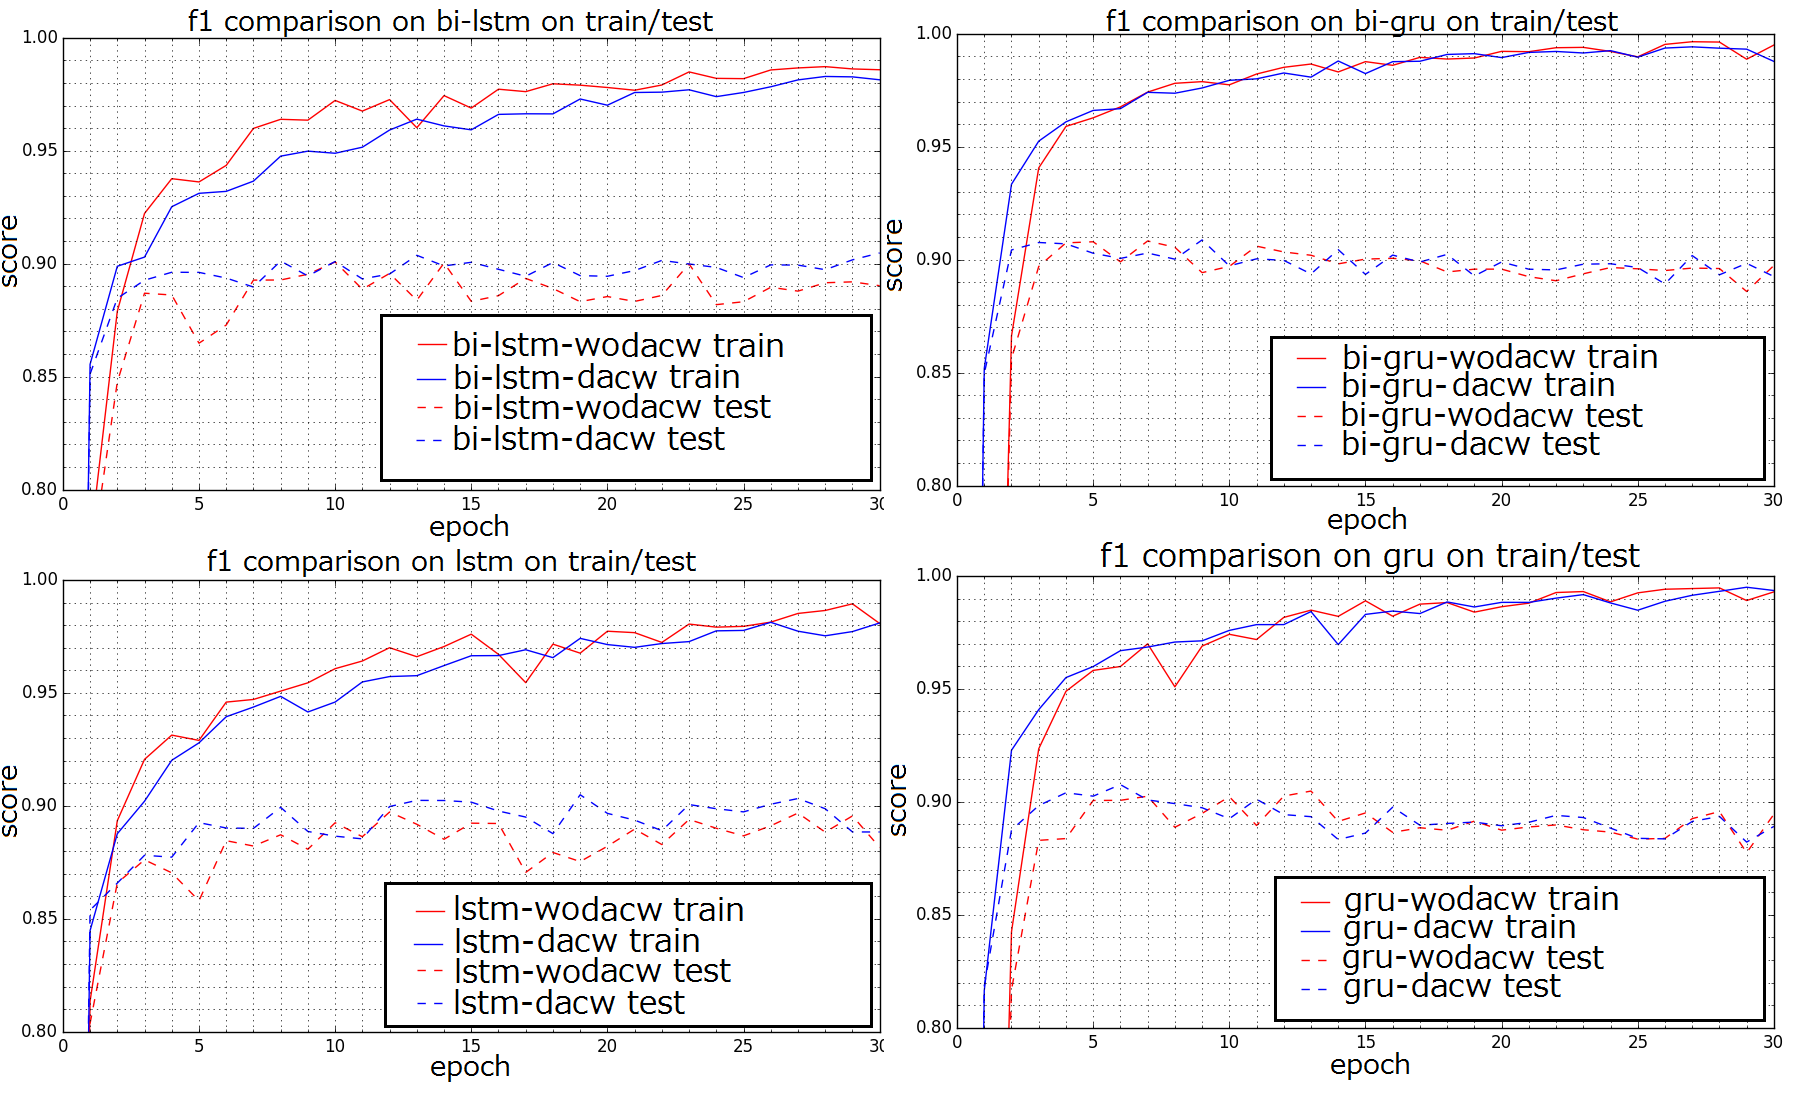
\includegraphics[scale=0.3]{image/5.png}
  \caption{Comparison between with and without DACW on different RNN models.}
  \label{fig:5}
\end{figure}
Figure~\ref{fig:5} illustrates the F1-score of the different models at each epoch.
``lstm'' and ``gru'' represents the model of RNN,
the prefix ``bi'' means bi-directional RNN, ``dacw'' and ``wodacw''
stand for the model with and without denoising autoencoder
with corrupted word (DACW).
The solid and break lines represent the results on the training
and test data, respectively.
Table~\ref{table:1} shows the average of F1-score between
$20^{th}-30^{th}$ epochs for simple comparison between
the model with and without DACW for single and bidirectional models.
\selectlanguage{english}
\begin{table}[ht]
\centering
%%%\tiny
\caption{Average of F1, precision, and recall for single/bi-directional
models with and without DACW.}
\label{table:1}

\scalebox{0.93}{
\begin{tabular}{|l|r|r|r|}
\hline
RNN model & pre-avg & recall-avg & f1-avg \\ \hline
lstm-wodacw & 0.8924 & 0.8896 & 0.8906 \\ 
gru-wodacw & 0.8885 & 0.8885 & 0.8873\\ 
bi-lstm-wodacw & 0.8934 & 0.8929 & 0.8923  \\ 
bi-gru-wodacw & 0.8953 & 0.8947 & 0.8936\\ \hline 
lstm-dacw & 0.8981 & 0.8966 & 0.8967\\ 
gru-dacw & 0.8899 & 0.8898 & 0.8894\\ 
bi-lstm-dacw & 0.8994 & 0.8996 & 0.8987\\ 
bi-gru-dacw & 0.8971 & 0.8964 & 0.8963\\ \hline 

\end{tabular}
}
\end{table}



From these results, we found that all bi-directional models provide better results
than single directional models.
One of the reasons is the flexibility of the word order in Thai language.
In English, the word order is almost always fixed as Subject-Verb-Object.
In contrast, both Subject-Verb-Object and Subject-Object-Verb are acceptable in Thai.
Moreover, an adjective can ap-pear before or after the head noun.
Since the word order in Thai is flexible,
bi-directional model may be appropriate to learn word sequence
and dependency between words that are useful for the classification.


Second, the models with DACW slightly out-performed the models without DACW.
The dif-ference between bi-lstm-dacw and bi-lstm-wodacw is verified by
McNemar's test. The p-value is 0.0003, indicating that the DACW can significantly
improve the F1 score.


\begin{figure}[!h]
\centering
  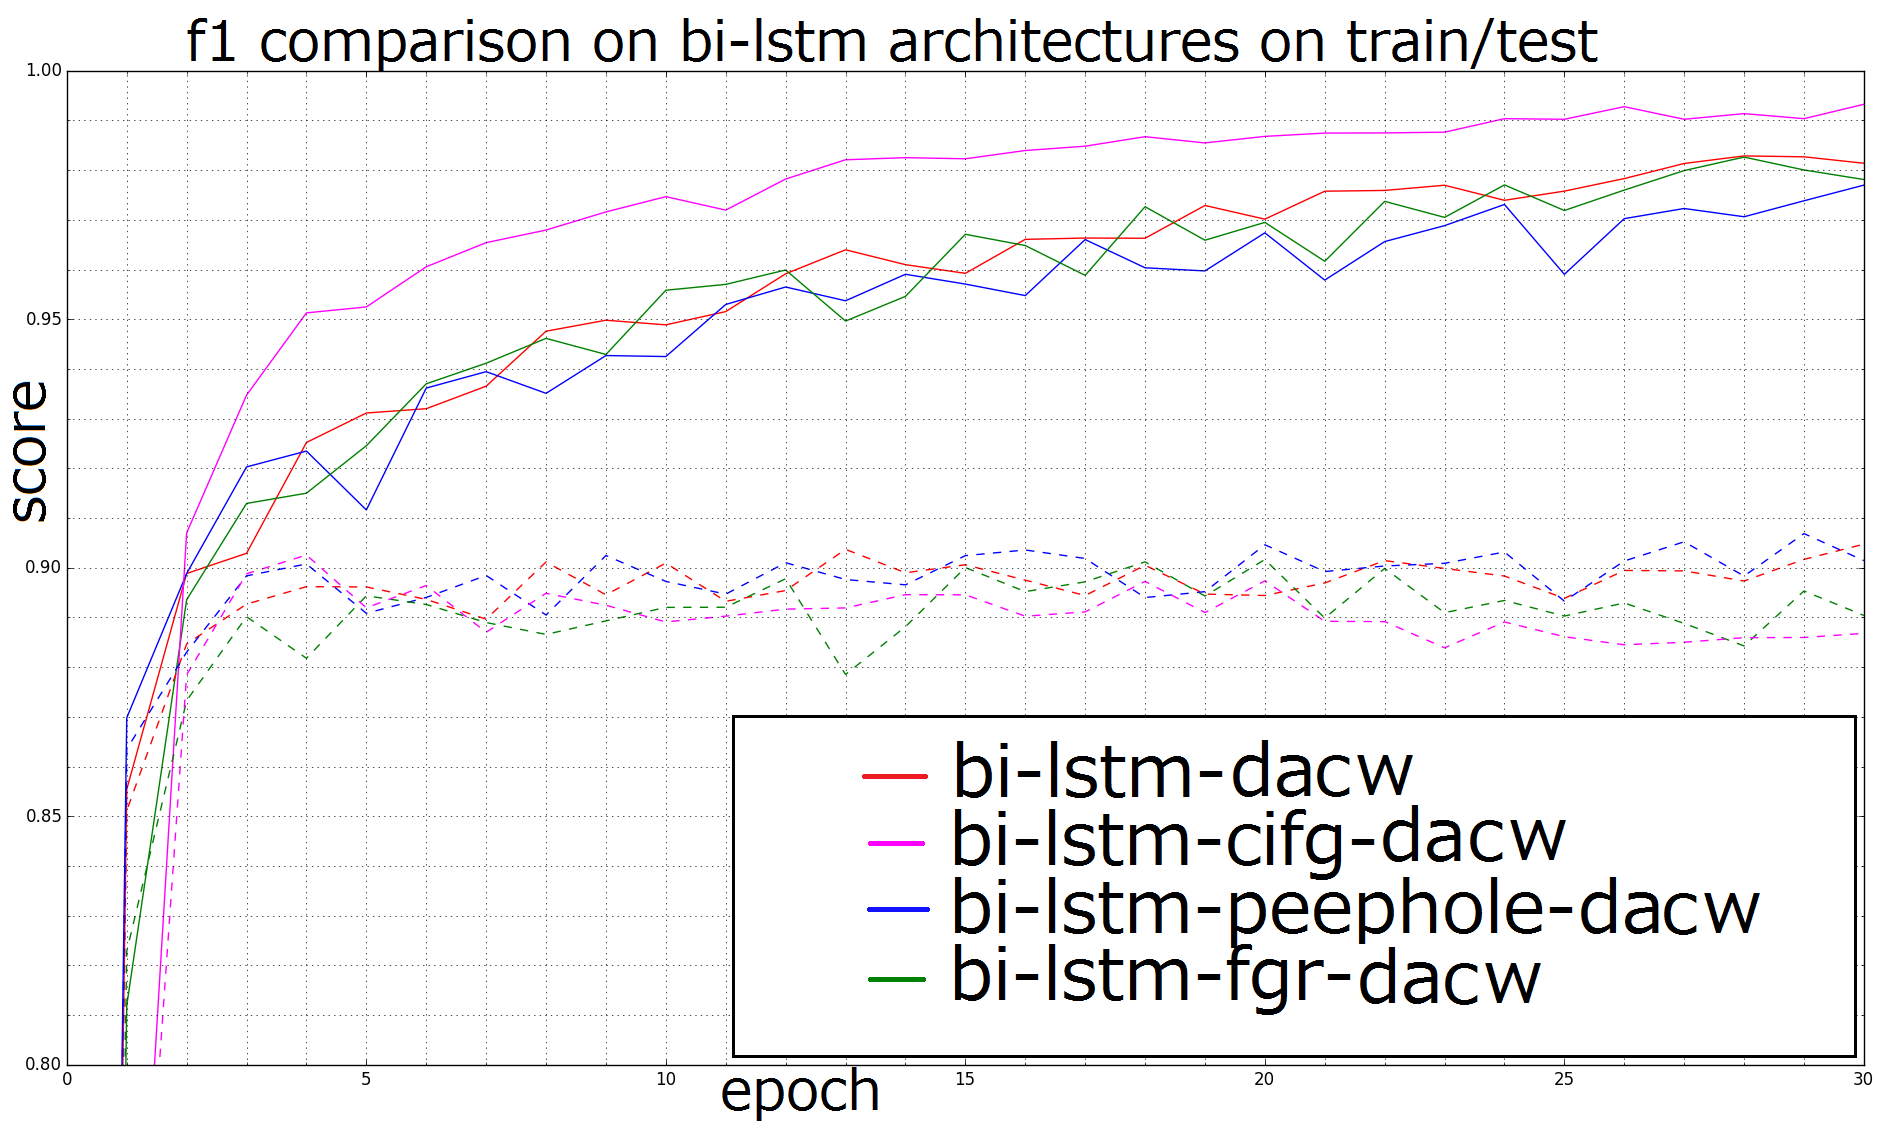
\includegraphics[scale=0.25]{image/6.png}
  \caption{Graph comparison among different bi-lstm architectures.}
  \label{fig:6}
\end{figure}
Since the best model was bi-lstm-dacw, we conduct further experiment by modifying
the LSTM gate to three other architectures: CIFG, peephole, and FGR.
Table~\ref{table:2} shows the average F1-score, while Figure~\ref{fig:6} 
shows the change of the F1-score against the number of epochs.
The solid and break lines represents the results on the training and test data,
respectively. 
Among all architectures, bi-lstm-cifg-dacw achieves the best 
result for a training set but underperforms on the test set
compared to other architectures. 
The bi-lstm-peephole-dacw provides the best result on the test set.
Meanwhile, the performance of bi-lstm-fgr-dacw is almost equivalent 
to the default architecture.
\selectlanguage{english}
\begin{table}[ht]
\centering
%%%\tiny
\caption{Average of F1, precision, and recall of differ-ent bi-lstm architectures.}
\label{table:2}

\scalebox{0.93}{
\begin{tabular}{|l|r|r|r|}
\hline
RNN model & pre-avg & recall-avg & f1-avg \\ \hline
bi-lstm-dacw & 0.8994 & 0.8996 & 0.8987 \\ 
bi-lstm-cifg-dacw & 0.8874 & 0.8871 & 0.8865 \\ 
bi-lstm-peephole-dacw & 0.9051 & 0.9039 & 0.9043 \\ 
bi-lstm-fgr-dacw & 0.8925 & 0.8922 & 0.8917 \\  \hline 

\end{tabular}
}
\end{table}



Table~\ref{table:3} shows the precision, recall and F1-score
for each of nine category.
Most remarkable point is that bi-lstm-peephole-dacw could perform much better
(by 0.1 F1-score) than bi-lstm-wodacw for ``Others'' category. 
Note that ``Others'' category is rather hard to be classified even
for human since a wide variety of the expressions are used.
The overall F1-score of bi-lstm-wodacw was suppressed by the poor performance
on ``Others'' category. 
Using denoising autoencoder with corrupted word and peephole gate,
now we achieved the F1-score more than 90\%.
\selectlanguage{english}
\begin{table}[ht]
\centering
%%%\tiny
\caption{Results of classification for each category.}
\label{table:3}

\scalebox{0.93}{
\begin{tabular}{|l|c|c|c|c|c|c|}
\hline
 & \multicolumn{3}{c|}{bi-lstm-peephole-dacw}& \multicolumn{3}{c|}{bi-lstm-wodacw}\\\cline{2-7}
category & precision & recall & f1 & precision & recall & f1 \\ \hline
Staff quality & 0.9371 & 0.9420 & 0.9395 & 0.8838 & 0.9623 & 0.9214 \\ 
Process & 0.9085 & 0.8910 & 0.8997 & 0.8827 & 0.9010 & 0.8918 \\
Accessibility & 0.8935 & 0.8580 & 0.8754 & 0.8365 & 0.8406 & 0.8386 \\ 
Facilities & 0.9265 & 0.9692 & 0.9474 & 0.9079 & 0.9388 & 0.9231 \\
Company brand & 0.8739 & 0.8899 & 0.8818 & 0.9820 & 0.8516 & 0.9121 \\
Product feature & 0.9182 & 0.8991 & 0.9085 & 0.9373 & 0.8557 & 0.8947 \\
Timing & 0.8345 & 0.8788 & 0.8561 & 0.8523 & 0.8141 & 0.8328 \\
Competitors & 0.9388 & 0.9388 &  0.9388 & 0.8793 & 0.8947 & 0.8870 \\
Others & 0.7826 & 0.7760 & 0.7742 & 0.7561 & 0.5962 & 0.6667 \\ \hline
avg/total &	0.9092 & 0.9091 & 0.9090 & 0.8947 & 0.8938 & 0.8927 \\ \hline

\end{tabular}
}
\end{table}


				



Finally, the contribution of the three components (preprocessing, DACW and peephole)
are shown in Table~\ref{table:4}.
``bi-lstm-no rule'' represents the bi-directional LSTM without
using preprocessing rules.
Comparing it with bi-lstm-wodacw, the rules improve the F1-score by 0.0582.
The contribution of DACW can be seen by the difference between bi-lstm-dacw
and bi-lstm-wodacw, which is 0.0064.
Similarly, the contribution of the peephole can be evaluated by comparison
between bi-lstm-dacw and bi-lstm-peephole-dacw (0.0056).
These results indicate that preprocessing of the text is important
since the contribution of the preprocessing rules is the most remarkable.
\selectlanguage{english}
\begin{table}[ht]
\centering
%%%\tiny
\caption{Contribution of three major components.}
\label{table:4}

\scalebox{0.93}{
\begin{tabular}{|l|r|r|r|}
\hline
RNN model & pre-avg & recall-avg & f1-avg \\ \hline
bi-lstm-no rule & 0.8303 & 0.8327 & 0.8341 \\ 
bi-lstm-wodacw & 0.8934 & 0.8929 & 0.8923 \\ 
bi-lstm-dacw & 0.8994 & 0.8996 & 0.8987 \\ 
bi-lstm-peephole-dacw & 0.9051 & 0.9039 & 0.9043 \\  \hline 

\end{tabular}
}
\end{table}






\subsection{Example}
Table~\ref{table:5} reveals several examples of the complaint classification.
The bold-underline characters mean the words or phrase that might
influence the prediction the most.
They are chosen from our intuition.
It shows that bi-lstm-wodacw cannot well handle an unseen word combination.
The phrase ``raise their tone'' and ``designed card'' in the third and
fourth sentences in Table~\ref{table:5} never appear in ``Staff quality'' and
``Others'' categories in the training sets.
While bi-lstm-wodacw failed to classify them correctly,
bi-lstml-peephole-dacw could do it thanks to its ability to handle
for the unseen words.
In the 5th sentence, the multiple use of the word ``slow'' suggests
that the category of this com-plaint is ``Timing'',
but its gold category is ``Process''.
The LSTM with peephole considers the number of times that the same 
word appears more heavily compared to the default LSTM. 
For the $6^th$ sentence, both models predict the category incorrectly 
since the phrase ``slow service'' is usually related to not 
``Timing'' but ``Staff quality''. 
Actually, this complaints may be related to both ``Timing'' and ``Staff quality''.
However, in our data set, only one category is annotated for each sentence.
Multiclass classification of the customer's complaints is an important future work.
\selectlanguage{english}
\begin{table}[ht]
\centering
\small
\caption{Examples of the complaint classification.}
\label{table:5}
\scalebox{0.525}{
\begin{tabular}{|l|c|c|c|c|}
\hline
Sentence & Gold label & bi-lstm-peephole-dacw & bi-lstm-wodacw & Evaluation remark \\ \hline
\multirow{ 2}{*}{}
\selectlanguage{thai}เจ้าหน้าที่|\_|มารยาท|\_|แย่|จัง| & & & &\\
The officer have a bad manner. & Staff quality & Staff quality & Staff quality & Correctly predicted\\ \hline
\selectlanguage{thai}ที่|อื่น|โปร|โมชั่น|ดี|กว่า|นี้|เยอะ|เลย|  &  &  &  &  \\
Other place given a better promotion. & Competitors & Competitors & Competitors & Correctly predicted \\ \hline
\selectlanguage{thai}ที่|นี่แหละ|ที่|callcenter|ไม่|ปลื้ม|เลย|ขึ้น|เสียง|แบบ| &  &  &  & \\ 
The callcenter always raise their tone. Don’t like it. & Staff quality & Staff quality & Timing & Clueless prediction on model two.  \\ \hline
\selectlanguage{thai}บัตร|ออกแบบ|มา|อย่าง|ปัญญาอ่อน| &  &  &  & \\
The designed card look retard. & Others & Others & Staff quality & Clueless prediction on model two. \\ \hline
\selectlanguage{thai}การแจ้ง|ผล|ช้า|ซะ|ยิ่ง|กว่า|ช้า| &  &  &  & \\
The notification process is slower than slowest. & Process & Timing & Process & Sensible prediction on model one. \\ \hline
\selectlanguage{thai}บริการ|ช้า|มาก|ทำ|เอา|ลูกค้า|ไม่|ปลื้ม| &  &  &  & \\
Customers are not happy from the very slow service. & Timing & Staff quality & Staff quality & Incorrectly predicted in the same manner. \\ \hline
\end{tabular}
}
\end{table}
